\documentclass[10pt, parskip=half-, twoside]{scrartcl}
\usepackage{castle_of_magic}
\usepackage[papersize={3.5in,5in}, margin=1cm]{geometry} % Set margins and footer placement

\usepackage{array}
\usepackage{enumitem}
\usepackage{multicol}

\usepackage{eso-pic}
\usepackage[skins]{tcolorbox} % Add background image to tikz node in color cover

\definecolor{lightbluestone}{HTML}{f3f7fd}
\definecolor{darkbluestone}{HTML}{d9ebf3}
\definecolor{paper}{HTML}{F1EBDB}

\usepackage{subcaption}

\usepackage{adjustbox}

\usepackage{float}

\usepackage[
	type={CC},
	modifier={by-nc-nd},
	version={4.0},
]{doclicense}

\usepackage[hidelinks]{hyperref}

% Adjust spacing before and after section headings
\RedeclareSectionCommand[
  runin=false,
  beforeskip=0.5\baselineskip,
  afterskip=-0.25\baselineskip
]{section}

% Adjust spacing before and after subsection headings
\RedeclareSectionCommand[
  runin=false,
  beforeskip=0.5\baselineskip,
  afterskip=-0.25\baselineskip
]{subsection}

% Adjust spacing before and after subsubsection headings
\RedeclareSectionCommand[
  runin=false,
  beforeskip=0.5\baselineskip,
  afterskip=-0.25\baselineskip
]{subsubsection}

% Adjust formatting of description environment
\setlist[description]{labelindent=0.25cm, leftmargin=\widthof{\hspace{0.25cm}\textbullet\space}, font=\normalfont\textbullet\bfseries\space}

% Adjust formatting of itemize environment
%itemize environments should be followed immediately by a \vspace{1ex} command.
%\setlist[itemize]{noitemsep,nolistsep,  leftmargin=0.68cm,topsep=-1ex}

\setkomafont{section}{\color{WildStrawberry}\LARGE\setmainfont{Tex Gyre Chorus}}
\setkomafont{subsection}{\color{WildStrawberry}\Large\setmainfont{TeX Gyre Chorus}}
\setkomafont{subsubsection}{\color{WildStrawberry}\large\setmainfont{TeX Gyre Chorus}}

\setmainfont{Charter}
\raggedright
\pagecolor{lightbluestone}
\begin{document}
{\contourlength{0.66pt}
\contournumber{256}
%\phantom{a}
\setmainfont[Scale=3.0]{Tex Gyre Chorus}
\center \Huge \contour{black}{\textcolor{WildStrawberry}{Castle}}

\contour{black}{\textcolor{WildStrawberry}{of}}

\contour{black}{\textcolor{WildStrawberry}{Magic}}
\vspace{0.25cm}
\contourlength{0.4pt}
\center \large \contour{black}{\textcolor{WildStrawberry}{The Card Game}}
\vfill
\setmainfont{Charter}
\contourlength{0.4pt}
\begin{center}
\Large Designed by Michael Purcell
\end{center}
%\center \contour{black}{\textcolor{WildStrawberry}{Designed  by Michael Purcell}}
%\phantom{a}
\AddToShipoutPictureBG*{
	\begin{tikzpicture}[remember picture, overlay]
		\draw[fill overzoom image=Images/blue_stone_wall_vector.png]  (current page.south west) rectangle (current page.north east);
	\end{tikzpicture}
}
}

\newpage
\AddToShipoutPictureBG{
	\begin{tikzpicture}[remember picture, overlay]
%		\draw[fill overzoom image=Images/blue_stone_wall_vector.png]  (current page.south west) rectangle (current page.north east);
		\draw[fill=darkbluestone]  (current page.south west) rectangle (current page.north east);

		\node[minimum height=5in-1cm, minimum width=3.5in-1cm, fill=lightbluestone, opacity=1.0, rounded corners=0.125in] () at (current page.center) {};
	\end{tikzpicture}
}

\section*{Background}
Thirty years ago, a group of adventurers journeyed to Castle Bondi to confront a Monster that lurked within.
Ultimately, they were able to perform a ritual spell and imprison the Monster.

The adventurers later established a network of twenty-seven shrines to channel the magical energies required to ensure that the Monster could not escape.% its prison.

Recently, three rival factions of wizards discovered how to corrupt the shrines.
%These factions began to use their power to control the kingdom in which the shrines are located.
As a result, the spell that binds the Monster has begun to falter.

Now, wizards from the three factions have come together to use the shrines to banish the Monster.
%If they succeed, their factions will vie for control of the kingdom.
If they fail, they risk releasing the Monster from its prison and being devoured as it rampages.

\newpage

\section*{Overview}
Castle of Magic: The Card Game is a game for 4-6 players that can be played in 30-60 minutes. It is intended for players who are at least twelve years old.

During the game, you will assume the role of a wizard who will try use the shrines to banish the Monster. You will have a set of secret objectives based on what faction you belong to and what country you are from.

To accomplish your objectives, you will manipulate the twenty-seven shrines. Whether you accomplish each of your objectives will depend on the state of the shrines at the end of the game.

The game will end when you cast the ritual spell. The fate of the Monster will depend on which version of the ritual spell you cast.

Your score will depend on how many of your objectives you accomplish. The players with the highest scores will win the game.

\newpage

\section*{Components}
\begin{itemize}[itemindent=*, leftmargin=*]
\item 65 Cards
	\begin{figure}[H]
	\centering
	\begin{subfigure}{0.4\textwidth}
	\centering
		
\includegraphics[scale=0.1]{Images/shrine_card_back.pdf}
	\caption*{27 Shrine Cards}
	\end{subfigure}
	\qquad
	\begin{subfigure}{0.4\textwidth}
	\centering
		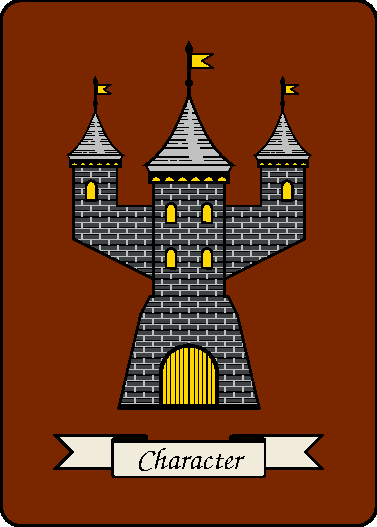
\includegraphics[scale=0.1]{Images/character_card_back.pdf}
	\caption*{13 Character Cards}
	\end{subfigure}
	\\[1em]
	\begin{subfigure}{0.4\textwidth}
	\centering
		
\includegraphics[scale=0.1]{Images/ritual_card_back.pdf}
	\caption*{8 Ritual Cards}
	\end{subfigure}
	\qquad
	\begin{subfigure}{0.4\textwidth}
	\centering
		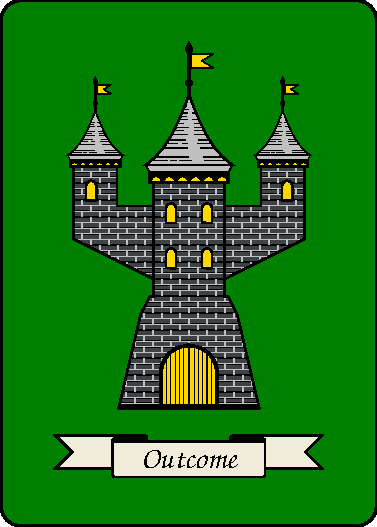
\includegraphics[scale=0.1]{Images/outcome_card_back.pdf}
	\caption*{8 Outcome Cards}
	\end{subfigure}
	\\[1em]
	\begin{subfigure}{0.4\textwidth}
	\centering
		
\includegraphics[scale=0.1]{Images/arcana_card_back.pdf}
	\caption*{6 Arcana Cards}
	\end{subfigure}
	\qquad
	\begin{subfigure}{0.4\textwidth}
	\centering
		
\includegraphics[scale=0.1]{Images/country_card_back.pdf}
	\caption*{3 Country Cards}
	\end{subfigure}
	\end{figure}
\vspace*{-1em}
\item 6 Player Aids
\begin{center}
%\hspace*{0.25cm}
\tikz{\pic[scale=0.1, transform shape] () at (0,0) {playeraiddisplaysmall={Red}};}
\hfill
\tikz{\pic[scale=0.1, transform shape] () at (0,0) {playeraiddisplaysmall={Orange}};}
\hfill
\tikz{\pic[scale=0.1, transform shape] () at (0,0) {playeraiddisplaysmall={kidagold}};}
\hfill
\tikz{\pic[scale=0.1, transform shape] () at (0,0) {playeraiddisplaysmall={dragongreen}};}
\hfill
\tikz{\pic[scale=0.1, transform shape] () at (0,0) {playeraiddisplaysmall={wolfblue}};}
\hfill
\tikz{\pic[scale=0.1, transform shape] () at (0,0) {playeraiddisplaysmall={hydrapurple}};}
\hspace*{0.25cm}
\end{center}
\item 12 Pawns (2 of each color)
\begin{center}
\hspace*{-0.25cm}
\tikz{\node () at (0,0) {
\includegraphics[width=0.25in]{Images/pawn_Red.png}};}
\hfill
\tikz{\node () at (0,0) {
\includegraphics[width=0.25in]{Images/pawn_Orange.png}};}
\hfill
\tikz{\node () at (0,0) {
\includegraphics[width=0.25in]{Images/pawn_kidagold.png}};}
\hfill
\tikz{\node () at (0,0) {
\includegraphics[width=0.25in]{Images/pawn_dragongreen.png}};}
\hfill
\tikz{\node () at (0,0) {
\includegraphics[width=0.25in]{Images/pawn_wolfblue.png}};}
\hfill
\tikz{\node () at (0,0) {
\includegraphics[width=0.25in]{Images/pawn_hydrapurple.png}};}
\hspace*{0.1cm}
\end{center}
\end{itemize}

\newpage

\phantom{a}
\vfill
\begin{figure}[ht]
\centering
\begin{adjustbox}{addcode={\begin{minipage}{\width}}{\caption*{%
      The play area after set up is complete.
      }\end{minipage}},rotate=-90,center}
\begin{tikzpicture}[x=1in, y=1in]
	\node[transform shape] () at (0,0) {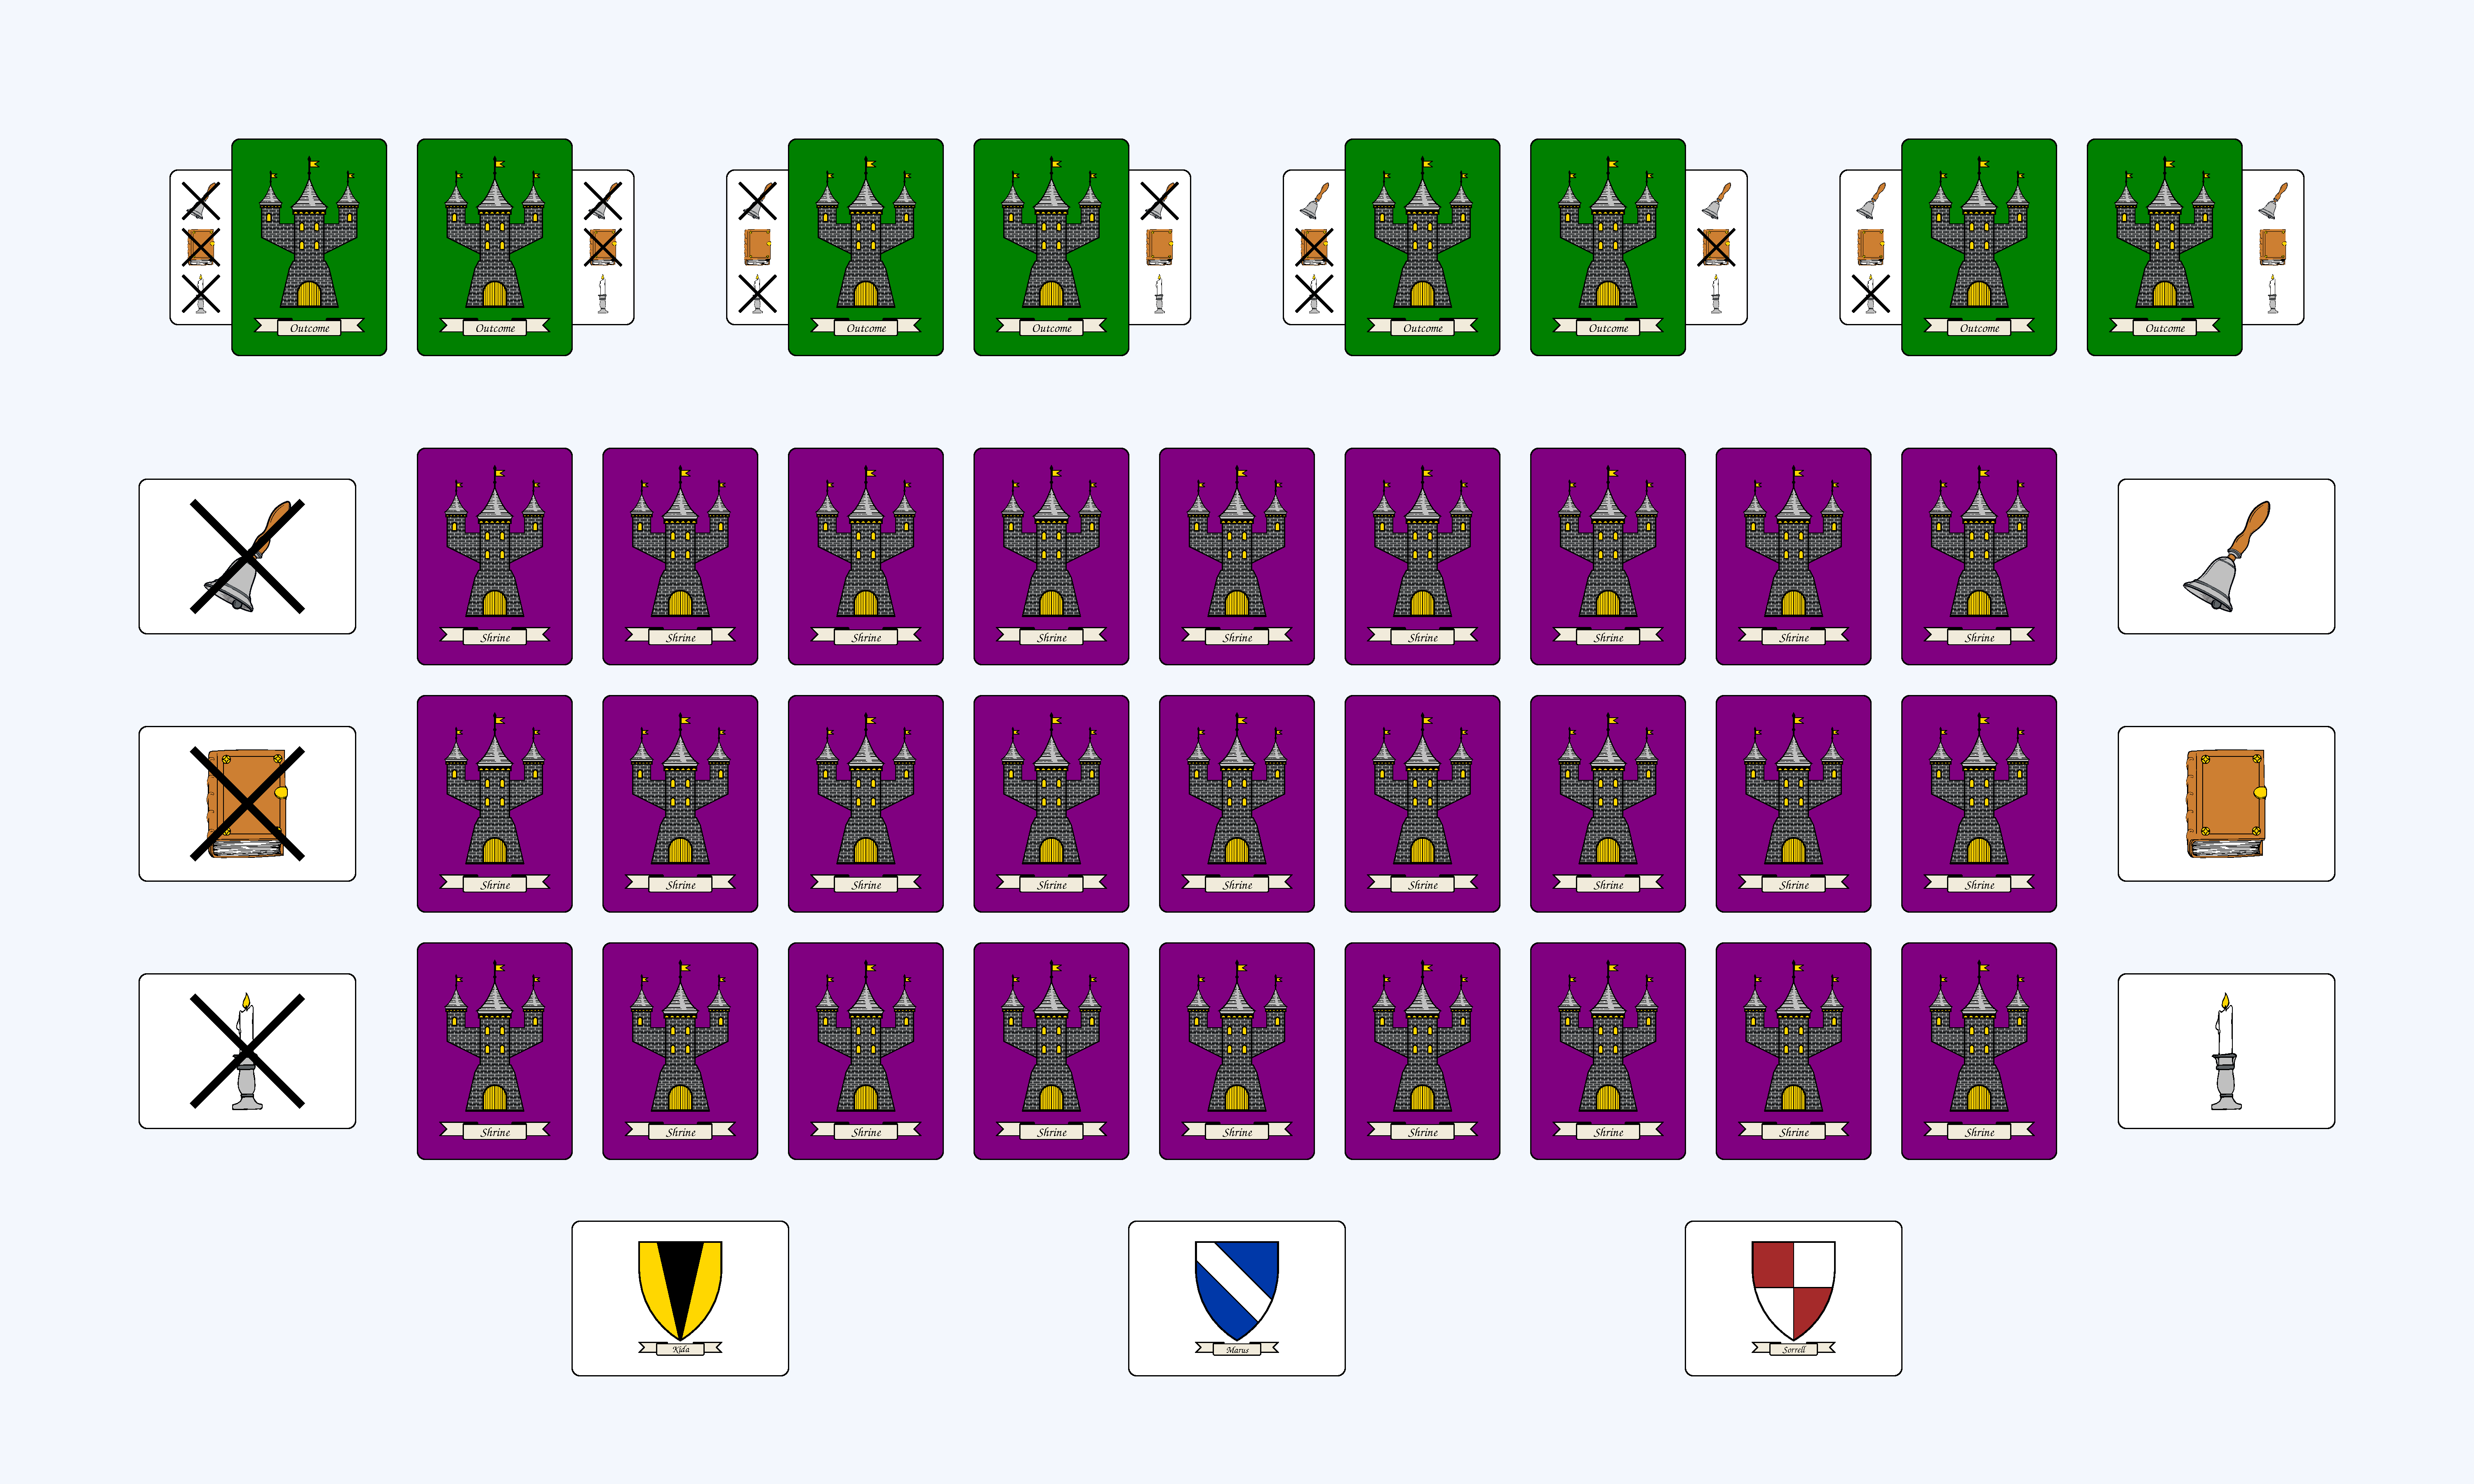
\includegraphics[scale=0.0775]{Images/play_area.pdf}};
\end{tikzpicture}
\end{adjustbox}
\end{figure}
\vfill
\phantom{a}

\newpage

\subsection*{Set Up}
\begin{enumerate}[itemindent=*, leftmargin=*]
	\item Assign each player a color. Give each player the pawns and the player aid that match their color.
	\item Shuffle the character cards.
	\item Deal a character card to each player.

	\item Shuffle the shrine cards.
	\item Arrange the shrine cards face down in a tableau consisting of three rows of nine cards each.
	\item Place the country cards below the tableau.
	\begin{enumerate}[itemindent=*, leftmargin=*]
		\item The Kida card should be placed below the second column.
		\item The Marus card should be placed below the fifth column.
		\item The Sorrell card should be placed below the eighth column.
	\end{enumerate}
	\item Place the arcana cards to the sides of the tableau. The cards for the inactive arcana (the ones with an ``X'' through them) should be placed on the left and the cards for the active arcana should be placed on the right of the tableau.
	\begin{enumerate}[itemindent=*, leftmargin=*]
		\item The bell cards should be placed next to the top row.
		\item The book cards should be placed next to the middle row.
		\item The candle cards should be placed next to the bottom row.
	\end{enumerate}
	\item Arrange the ritual cards face up in a single row above the tableau.
	\item Shuffle the outcome cards.
	\item Place one outcome card on top of each ritual card. Ensure that the icons on the ritual cards remain visible.
\end{enumerate}

\newpage

\section*{Playing the Game}
The player who has most recently performed a magic trick should take the first turn.

On your turn you must either manipulate the shrines or advance the ritual spell. Each player must manipulate the shrines on their first turn.

Play proceeds to the left (clockwise). That is, when you have finished your turn, the player to your left will take the next turn.

Play continues this way until the ritual spell is cast and the game ends.

After the game ends, you will identify which objectives you accomplished and compute your total score. The players with the highest scores will win the game.

\newpage
 
\subsection*{Manipulating the Shrines}
To manipulate the shrines, you must pick up at least one of your pawns.

For every pawn that you picked up you must:
	\begin{enumerate}[itemindent=*, leftmargin=*]
	\item Flip one shrine card that does not have a pawn on it.
	\item Place a pawn that you picked up on the shrine card that you flipped.
	\end{enumerate}

\subsection*{Advancing the Ritual Spell}
To advance the ritual spell, you must flip one of the face down outcome cards so that it is face up.
	
\subsection*{Ending the Game}
The game ends immediately when the last ritual card is turned face up.

\newpage

\section*{Factions}
Three factions of wizards - the Dragon Masters, the Eagle Lords, and the Wolf Mages - have come together to cast the ritual spell. They are also political rivals.

Each faction has corrupted eight of the twenty-seven shrines. They will use these shrines to vie for control of the kingdom.
\vfill
\begin{figure}[hb]
\centering
\begin{subfigure}{0.4\textwidth}
\centering
\begin{tikzpicture}
	\pic[transform shape, scale=0.35, yshift=0.25] () at (0,0) {dragon};
	\path (0,-1.15) -- (0,1.15);
\end{tikzpicture}
\caption*{Dragon Masters}
\end{subfigure}
\quad
\begin{subfigure}{0.4\textwidth}
\centering
\begin{tikzpicture}
	\pic[transform shape, scale=0.35] () at (0,0) {wolf};
	\path (0,-1.15) -- (0,1.15);
\end{tikzpicture}
\caption*{Wolf Mages}
\end{subfigure}
\\[1em]
\begin{subfigure}{0.4\textwidth}
\centering
\begin{tikzpicture}
	\pic[transform shape, scale=0.35] () at (0,0) {eagle};
\end{tikzpicture}
\caption*{Eagle Lords}
\end{subfigure}
\caption*{Sigils of the three factions of wizards.}
\end{figure}


\newpage

\section*{Countries}
Three countries - Kida, Marus, and Sorrell - comprise the kingdom and are where the twenty-seven shrines are located. Nine shrines are in each country.

When the ritual spell is cast, each country will be controlled by the faction with the most active shrines in that country.
\vfill
{
\begin{figure}[hb]
\centering
\begin{subfigure}{0.35\textwidth}
\centering
\begin{tikzpicture}
	\pic[transform shape, scale=0.175] () at (0,0) {simplecoa={Kida}};
\end{tikzpicture}
\caption*{Kida}
\end{subfigure}
\quad
\begin{subfigure}{0.35\textwidth}
\centering
\begin{tikzpicture}
	\pic[transform shape, scale=0.175] () at (0,0) {simplecoa={Marus}};
\end{tikzpicture}
\caption*{Marus}
\end{subfigure}
\\[0.5em]
\begin{subfigure}{0.35\textwidth}
\centering
\begin{tikzpicture}
	\pic[transform shape, scale=0.175] () at (0,0) {simplecoa={Sorrell}};
\end{tikzpicture}
\caption*{Sorrell}
\end{subfigure}
\setmainfont{Charter}
\caption*{Coats of Arms for the three countries.}
\end{figure}
}
\newpage

\section*{Regalia}
Three pieces of regalia - the amulet, the crown, and the scepter - were originally used to control the Monster. Each piece of regalia was interred within one of the twenty-seven shrines when the Monster was imprisoned. Now, the regalia are treasures that the wizards can claim to further their personal ambitions.

When the ritual spell is cast, any character who has claimed a piece of regalia may draw the attention of the Monster. They may be able to to used the regalia to dominate the Monster but risk being devoured if the Monster is released.
\vfill
\begin{figure}[hb]
\centering
\begin{subfigure}{0.3\textwidth}
\centering
\begin{tikzpicture}
	\pic[transform shape, scale=0.35] () at (0,0) {amulet};
	\path (0,-1.25) -- (0,1.25);
\end{tikzpicture}
\caption*{Amulet}
\end{subfigure}
\hfill
\begin{subfigure}{0.3\textwidth}
\centering
\begin{tikzpicture}
	\pic[transform shape, scale=0.35] () at (0,0) {crown};
	\path (0,-1.25) -- (0,1.25);
\end{tikzpicture}
\caption*{Crown}
\end{subfigure}
\hfill
\begin{subfigure}{0.3\textwidth}
\centering
\begin{tikzpicture}
	\pic[transform shape, scale=0.35] () at (0,0) {scepter};
	\path (0,-1.25) -- (0,1.25);
\end{tikzpicture}
\caption*{Scepter}
\end{subfigure}
%\caption*{The three regalia.}
\end{figure}

\newpage

\section*{Arcana}
Three arcana - the bell, the book, and the candle - were originally used to summon the Monster. Now, the wizards will harness the power of the arcana to cast the ritual spell.

The nature of the ritual spell will depend on how each of of the arcana are used when it is cast. Each of the arcana can be used in one of two ways:
\begin{itemize}[itemindent=*, leftmargin=*]
\item The bell can be either ringing or silent.
\item The book can be either open or closed.
\item The candle can be either lit or unlit.
\end{itemize}
So, there are eight possible outcomes when the ritual spell is cast.
\vfill
\begin{figure}[hb]
\centering
\begin{subfigure}{0.3\textwidth}
\centering
\begin{tikzpicture}
	\pic[transform shape, scale=0.35, rotate=-90] () at (0,0) {bell};
	\path (0,-1.25) -- (0,1.25);
\end{tikzpicture}
\caption*{Bell}
\end{subfigure}
\hfill
\begin{subfigure}{0.3\textwidth}
\centering
\begin{tikzpicture}
	\pic[transform shape, scale=0.35, rotate=-90] () at (0,0) {book};
	\path (0,-1.25) -- (0,1.25);
\end{tikzpicture}
\caption*{Book}
\end{subfigure}
\hfill
\begin{subfigure}{0.3\textwidth}
\centering
\begin{tikzpicture}
	\pic[transform shape, scale=0.35, rotate=-90] () at (0,0) {candle};
	\path (0,-1.25) -- (0,1.25);
\end{tikzpicture}
\caption*{Candle}
\end{subfigure}
%\caption*{The three regalia.}
\end{figure}

\newpage

\section*{The Twenty-Seven Shrines}
The twenty-seven shrines were built to channel the magical energies required to imprison the monster. Each shrine is attuned to one of the three arcana and is located in one of the three countries.

Each shrine is represented by a shrine card.
If a shrine card is face up, the corresponding shrine is active.
If a shrine card is face down, the corresponding shrine is inactive.

\subsection*{Corrupted Shrines}
Most of the shrines have been corrupted by one of the three factions. Only the shrines in which the regalia are interred have not been corrupted.

The factions can use the shrines that they have corrupted to exert control over the countries in which those shrines are located.

\newpage

\subsection*{The Tableau}
The shrine cards will be arranged in a tableau consisting of three rows of nine cards each.

Each row of the tableau will contain the cards that represent the shrines that are attuned to one of the arcana.
\begin{itemize}[itemindent=*, leftmargin=*]
\item The top row is for the bell.
\item The middle row is for the book.
\item The bottom row is for the candle.
\end{itemize}

The columns of the tableau contain the cards that represent the shrines that are located in one of the three countries.
\begin{itemize}[itemindent=*, leftmargin=*]
\item The first three columns are for Kida.
\item The next three columns are for Marus.
\item The last three columns are for Sorrell.
\end{itemize}

%Each shrine can be either active or inactive.
%\begin{itemize}[itemindent=*, leftmargin=*]
%\item If a shrine card is face up, the corresponding shrine is active.
%\item If a shrine card is face down, the corresponding shrine in inactive.
%\end{itemize}

%\newpage


\newpage

\section*{The Ritual Spell}
The game ends when the wizards cast the ritual spell. The nature of the ritual spell depends on how each of the arcana are used when it is cast.

How each each of the arcana is used depends on the state of the shrines that are attuned to that arcanum.
\begin{itemize}[itemindent=*, leftmargin=*]
\item If the majority (five or more) of the shrines in the top row of the tableau are active, the bell is ringing. Otherwise, the bell is silent.
\item If the majority (five or more) of the shrines in the middle row of the tableau are active, the book is open. Otherwise, the bell is closed.
\item If the majority (five or more) of the shrines in the bottom row of the tableau are active, the candle is lit. Otherwise, the candle is unlit.
\end{itemize}

\newpage

\subsection*{Determining the Outcome}
There are eight possible ritual spells.
The ritual spell that is cast depends on how the arcana are used.
Each ritual spell is represented by a ritual card.

Each outcome describes what happens when one of the ritual spells is cast. 
Each outcome is represented by an outcome card.

The mapping between outcomes and ritual spells changes from game to game. The outcome cards specify which outcome corresponds to which ritual spell.

\subsection*{Casting the Ritual Spell}
At the beginning of the game, all of the outcome cards will be face down. During the game, players will have the opportunity to turn the outcome cards face up.

The ritual spell is cast immediately when the last outcome card is turned face up.

\newpage

\subsection*{Outcomes}
There are eight possible outcomes when the ritual spell is cast.
\begin{enumerate}[itemindent=*, leftmargin=*]
\item The character who claimed the amulet dominates the Monster.% If no one claimed the amulet then the Monster is released. Everyone is devoured as the Monster rampages.
\item The character who claimed the crown dominates the Monster.% If no one claimed the crown then the Monster is released. Everyone is devoured as the Monster rampages.
\item The character who claimed the scepter dominates the Monster.% If no one claimed the scepter then the Monster is released. Everyone is devoured as the Monster rampages.
\item The character who claimed the amulet is devoured by the Monster.%Afterwards, the Monster is banished.
\item The character who claimed the crown is devoured by the Monster. %Afterwards, the Monster is banished.
\item The character who claimed the scepter is devoured by the Monster.%Afterwards, the Monster is banished.
\item The Monster is released. Everyone is devoured as the Monster rampages.
\item The Monster is banished outright.
\end{enumerate}

\newpage
%\topskip0pt
%\vspace*{\fill}
\begin{figure}[H]
\centering
\begin{subfigure}{0.3\textwidth}
\centering
\begin{tikzpicture}
	\pic[transform shape, scale=0.35, yshift=0.25] () at (0,0) {amulet_laurel};
	\path (0,-1.0) -- (0,1.0);
\end{tikzpicture}
\caption*{Outcome 1.}
\end{subfigure}
\hfill
\begin{subfigure}{0.3\textwidth}
\centering
\begin{tikzpicture}
	\pic[transform shape, scale=0.35] () at (0,0) {crown_laurel};
	\path (0,-1.0) -- (0,1.0);
\end{tikzpicture}
\caption*{Outcome 2.}
\end{subfigure}
\hfill
\begin{subfigure}{0.3\textwidth}
\centering
\begin{tikzpicture}
	\pic[transform shape, scale=0.35] () at (0,0) {scepter_laurel};
	\path (0,-1.0) -- (0,1.0);
\end{tikzpicture}
\caption*{Outcome 3.}
\end{subfigure}
\\[1.25em]
\begin{subfigure}{0.3\textwidth}
\centering
\begin{tikzpicture}
	\pic[transform shape, scale=0.35] () at (0,0) {amulet_dead};
	\path (0,-1.0) -- (0,1.0);
\end{tikzpicture}
\caption*{Outcome 4.}
\end{subfigure}
\hfill
\begin{subfigure}{0.3\textwidth}
\centering
\begin{tikzpicture}
	\pic[transform shape, scale=0.35] () at (0,0) {crown_dead};
	\path (0,-1.0) -- (0,1.0);
\end{tikzpicture}
\caption*{Outcome 5.}
\end{subfigure}
\hfill
\begin{subfigure}{0.3\textwidth}
\centering
\begin{tikzpicture}
	\pic[transform shape, scale=0.35] () at (0,0) {scepter_dead};
	\path (0,-1.0) -- (0,1.0);
\end{tikzpicture}
\caption*{Outcome 6.}
\end{subfigure}
\\[1.25em]
\begin{subfigure}{0.5\textwidth}
\centering
\begin{tikzpicture}
	\pic[transform shape, scale=0.35] () at (0,0) {hydra};
\end{tikzpicture}
\caption*{Outcome 7.}
\end{subfigure}
\hfill
\begin{subfigure}{0.45\textwidth}
\centering
\begin{tikzpicture}
	\pic[transform shape, scale=0.35] () at (0,0) {hydra_dead};
\end{tikzpicture}
\caption*{Outcome 8.}
\end{subfigure}
\caption*{Icons that represent each of the eight possible outcomes of the ritual spell.}
\end{figure}

\newpage

\section*{Characters}
There are three kinds of characters: wizards, cultists, and the Monster.

\subsection*{Wizards}
Each wizard is affiliated with both a faction and a country. Each wizard's affiliations are represented in the form of a coat of arms.

The shield in a wizard's coat of arms indicates the country that they are from. The supporters in a wizard's coat of arms indicate their faction.

\subsection*{Cultists}
Each cultist is affiliated with a faction. Cultists are not affiliated with any country. Instead, cultists worship the Monster. Each cultist's affiliations are represented in the form of a coat of arms.

The shield in a cultists coat of arms bears the image of the Monster. The supporters in a cultist's coat of arms indicate their faction.

\newpage

\subsection*{The Monster}
The Monster has the ability to disguise itself as a wizard. If you are the Monster, then you can manipulate the shrines and the ritual cards as normal.

The only mechanical difference between the Monster and a wizard or a cultist during the game is that they have different objectives.

\vfill

\begin{figure}[hb]
\centering
\begin{tikzpicture}
	\pic[scale=0.75, transform shape] () at (0,0) {hydra};
\end{tikzpicture}
\caption*{The Monster}
\end{figure}

\newpage

\section*{Objectives}
There are four types of objectives that you (or others) may be trying to accomplish: controlling countries, claiming regalia, dominating the monster, and feeding the Monster.

\subsection*{Controlling Countries}
To control each country, you will need to ensure that your faction has the most active shrines in that country. If two or more of the factions are tied for the most active shrines in a country, then none of the factions will control that country.

\subsection*{Claiming Regalia}
To claim a piece of regalia, one of your pawns must be on its shrine card when the ritual spell is cast. You can claim a piece of regalia regardless of whether its shrine card is face up or face down.

\newpage

\subsection*{Dominating the Monster}
To dominate the Monster, you must first claim a piece of regalia. Then, you must ensure that the outcome of the ritual spell allows you dominate the Monster.

\subsection*{Feeding the Monster}
To feed the Monster, you must ensure that the outcome of the ritual spell indicates that the Monster devours at least one character.

\newpage

\section*{Scoring}
Each type of character scores points based on what objectives they are able to accomplish.

\subsection*{Wizards}
Each wizard scores:
\begin{itemize}[itemindent=*, leftmargin=*]
\item 1000 points for every country that their faction controls.
\item 1000 points for their faction controlling their home country.
\item 1000 points for every piece of regalia that they claim.
\item 1000 points for dominating the Monster.
\end{itemize}
A wizard who is devoured by the Monster cannot claim any of the regalia.

\newpage

\subsection*{Cultists}
Each cultist scores:
\begin{itemize}[itemindent=*, leftmargin=*]
\item 1000 points for each country that their faction controls.
\item 1000 points for each piece of regalia that they claim.
\item 1000 points for feeding the Monster.
\end{itemize}
A cultist who is devoured by the monster cannot claim any of the regalia.

\subsection*{The Monster}
The Monster scores:
\begin{itemize}[itemindent=*, leftmargin=*]
\item 6000 points for devouring at least one wizard or cultist.
\end{itemize}
The Monster can claim regalia but will not score points for doing so. The Monster cannot devour itself.

\newpage

\section*{Playtesters}
The design of Castle of Magic: The Card Game has been vastly improved by the feedback provided by the following playtesters throughout the design process:
\begin{multicols}{2}
\begin{itemize}%[nosep]
\item Dannielle Harden
\item Luke Purcell
\item Kira Purcell
\item Farzana Choudhury
\item Keydan Bruce
\item Brett Witty
\end{itemize}
\end{multicols}

\section*{Design Tools}
The following tools were used to create the art, layout, and graphic design for this game:
\begin{description}[font=\normalfont\textbullet\space, nosep]
	\item[LuaLaTeX:] Typesetting and layout.
	\item[TikZ:] Diagrams and art.
	\item[GIMP:] Image manipulation.
\end{description}
\vspace{1ex}
The fonts used in this booklet are Charter and TeX Gyre Chorus.

The art used throughout the game was adapted from illustrations by d3verro.

\newpage

\section*{Disclaimer}
This game is a modern reimagining of a classic board game of magic and intrigue.

The original Castle of Magic game was designed by Rick Smith and published by Cloud Kingdom Games (n\'ee RiddleMaster Games) in 1991. 

It was later augmented by two expansions: The Castle Cursed in 1992 and The Fall of Castle Bondi (which includes a reprint of the earlier expansion) in 2002.

Castle of Magic: The Card Game was designed by Michael Purcell. It is an original design that aims to maintain the flavor of the original while simplifying it for a more streamlined experience.  

Rick Smith holds all rights to Castle of Magic, and this work has been made available for print-and-play and low-volume print-on-demand with his permission. 

\vfill
\textbf{Contact}: \href{mailto:castle.of.magic.tcg@gmail.com}{castle.of.magic.tcg@gmail.com}\\
\begin{tabular}{@{}m{\textwidth-\widthof{\Huge{\doclicenseIcon}}}@{\hspace*{0.5cm}}m{\widthof{\Huge{\doclicenseIcon}}-0.5cm}@{}}
\footnotesize{\doclicenseText} & \huge{\doclicenseIcon} \\
\end{tabular}

\newpage

\AddToShipoutPictureBG*{
	\begin{tikzpicture}[remember picture, overlay]
		\draw[fill overzoom image=Images/blue_stone_wall_vector.png]  (current page.south west) rectangle (current page.north east);
	\end{tikzpicture}
}
\begin{figure}[ht]
\centering
\begin{tikzpicture}
	\pic[scale=1.55, transform shape] () at (0,0) {castle};
\end{tikzpicture}
%\caption*{Castle Bondi: The Castle of Magic}
\end{figure}

\end{document}
